% !TeX spellcheck = en_US


\documentclass[10pt,a4paper]{article}
\usepackage{lrec}
\usepackage{multibib,filecontents}
%\newcites{languageresource}{Language Resources}
\usepackage{tablefootnote}
\usepackage{times}
\usepackage{graphicx}
\usepackage{tabularx,multirow}
\usepackage{soul}
\usepackage[ruled]{algorithm2e}
% for eps graphics

\usepackage{tipa}
\let\ipa\textipa
\usepackage{vowel,amssymb}

%\usepackage{epstopdf}
%\usepackage[latin1]{inputenc}

\usepackage{fontspec}
\setmainfont{FreeSerif}
%\setmainfont{TeX Gyre Termes}
\usepackage{polyglossia}
\setmainlanguage{english}
\setotherlanguages{sanskrit} %% or other languages
\newfontfamily\devanagarifont[Script=Devanagari]{Annapurna SIL}
\newcommand{\sansk}[1]{\begin{sanskrit}#1\end{sanskrit}}

\usepackage[
pdfauthor={Aalok Sathe},
pdftitle={A Rule-Based System for the Transcription of Sanskrit from the Devanagari Orthography to the International Phonetic Alphabet},
pdfsubject={Linguistics},
pdfkeywords={Transcription, Sanskrit, IPA, Phonetics, WWG algorithm, Devanagari, Computational linguistics},
pdfproducer={XeLaTeX },
pdfcreator={xelatex}TimesNewRoman]{hyperref}

%\usepackage{xstring}

%\newcommand{\secref}[1]{\StrSubstitute{\getrefnumber{#1}}{.}{ }}

\title{A Rule-Based System for the Transcription of Sanskrit from the Devanagari Orthography to the International Phonetic Alphabet}

\name{Aalok Sathe}

\address{University of Richmond
	\\28 Westhampton Way, Richmond, VA 23173, USA
	\\
    \hyperref{mailto:aalok.sathe@richmond.edu}{}{}{aalok.sathe@richmond.edu}\\}


\abstract{
	We propose a new system for the transcription of Sanskrit text written using the Devanagari orthography, into the International Phonetic Alphabet, and supplement it with free and open-source software. We make use of existing literature on closest known pronunciations of sounds as well as prosodic and metric rules of syllabification using the Weerasinghe-Wasala-Gamage (WWG) algorithm for Sinhala, adapted to Sanskrit. We further incorporate suprasegmental sound changes along with the assignment of syllable-weight-determined stress.
\\
\newline \Keywords{Transcription, Sanskrit, IPA, Phonetics, WWG algorithm, Devanagari, Computational linguistics} }

\begin{document}

\maketitleabstract

\section{Introduction}

The language Sanskrit is one of the oldest classical languages, and has a large amount of literature. For this reason, Sanskrit is a topic of frequent study in literature, culture, and linguistics. One hurdle in this process of studying is often the lack of an all-encompassing system of phonetic transcription. Whereas the IAST\footnote{International Alphabet of Sanskrit Transliteration} and ITRANS\footnote{Indian languages TRANSliteration} are widely used today, and will continue to be, they are but alternate means of representation of the same text, not fully capturing the phonological and prosodic features of the language. Additionally, it is our personal experience that even though systems such as IAST exist, students of Sanskrit worldwide have varying pronunciations of the same few sounds, seemingly approximated to the inventory of their primary languages. For new learners or even existing scholars, there can be a steep learning curve in Sanskrit phonology. Hence, it would be beneficial to new learners to have a system that would guide pronunciation as accurately and consistently as possible. 


Some newer tools seemingly try to address this issue. However, they either do not solve the problem at hand, or do so inaccurately. Examples include the `ICU' system for transliteration of Indic scripts \cite{viswanadha2002transliteration} as well as the website ``Ashtangayoga'' \cite{ashtangayoga}. In the case of the latter, we notice a lack of any indication of stress, syllabification, as well as that of within-word and suprasegmental phonological phenomena whatsoever. One may disregard these as `superficial' details, but they are far from being that as syllabification and stress play an important role in classical Sanskrit poetic composition. We propose an improved system, hence, which we hope will serve as a convenient tool for reference in the study of Sanskrit phonology. 
We describe a system for the transcription of Sanskrit text written using its Devanagari orthography into the international phonetic alphabet (IPA). We choose IPA in particular to enable near-completeness of representation of the best-known pronunciations of Sanskrit sounds, rule-based syllabification adapted for Sanskrit from the Weerasinghe-Wasala-Gamage algorithm (`WWG algorithm') originally developed for the Sinhala language, and syllable stress: a prosodic feature not captured in any modern transcription system (e.g., IAST).

In this work, we aim to develop, based on existing work, a rule-based algorithmic system, and a computer program to supplement it, which will provide a consistent transcription given well-formed\footnote{That is, one adhering to the rules of classical Sanskrit phonology and Devanagari orthography} Sanskrit text.
We develop and distribute software accompanying this system, and license it using the GNU General Public License 3, to enable anyone to access and redistribute the source code as well as develop other software with the current implementation at its base. We believe this software will in itself be a tool for preservation of traditional knowledge as well as help create newer ones.


\section{Sanskrit Phonology}

Sanskrit is a classical language with its origins in the Indian subcontinent, and its literature and texts being found in present-day India, Nepal, and neighboring regions.
Sanskrit is one of the official languages of India and shares close common ancestry with most of the modern Indo-Aryan languages spoken in the Indian subcontinent today \cite{emeneau1956india} as well as some of the older Indo-European languages. It was recorded as the mother-tongue of about 14,000 people in the 2001 census of India \cite{banthia2001census}. While the effective pronunciations of Sanskrit sounds differ from region to region depending on the speaker's own mother tongue and regional linguistic influence, a unified approximation of Sanskrit sounds has been proposed in several existing works based on historical as well as present-day phonetic studies. In what follows, we attempt to give a summary of Sanskrit speech sounds.

\begin{table*}[ht]
	\centering
	
	\begin{center}
		\begin{tabular}{|c|l|l|l|}
			\hline
			&Front&Central&Back\\\hline
			High&\sansk{इ} ([i]), \sansk{ई} ([iː])&&\sansk{उ} ([u]), \sansk{ऊ} ([uː])\\
			Mid&$\phi$,$\hskip0.em\quad\quad$\sansk{ए} ([eː])&\sansk{अ} ([ə]), $\phi$ &$\phi$,$\hskip0.em\quad\quad$ \sansk{ओ} ([oː])\\
			Low&&$\phi$,$\quad\quad$ \sansk{अा} ([ɑː])&\\
			\hline				
		\end{tabular}
		\caption{Sanskrit speech sounds: simple vowels. Symbols on the left are short variants of the vowel, while those on the right are long. In case a variant of a vowel does not exist, `$\phi$' is shown. Blanks denote vowels not in the Sanskrit phoneme inventory.}
		\label{vowel-positions-chart}
	\end{center}
\end{table*}

\begin{table}[]
	\centering
	
	\begin{center}
		\begin{tabular}{|c|c|c|}
			\hline
			$X$&$X+$\sansk{इ,ए}&$X+$\sansk{उ,अो}\\\hline
			\sansk{अ,अा}&\sansk{ऐ} ([ɑːi])&\sansk{औ} ([ɑːu])\\\hline
			
		\end{tabular}
		\caption{Sanskrit speech sounds: simplified rules of diphthong formation}
		\label{diphthongs-table}
	\end{center}
	%	\label{diphth}
\end{table}

\begin{table}[]
	\centering
	
	\begin{center}
		\begin{tabular}{|c|}
			\hline
			\sansk{ऋ} ([ɹ̩]),$\quad$ \sansk{ॠ} ([ɹ̩ː])\\\hline\hline
			\sansk{ऌ} ([l̩]),$\quad$ \sansk{ॡ} ([l̩ː])\\\hline
			
		\end{tabular}
		\caption{Sanskrit speech sounds: special vowels (sonorants). The first row shows short and long syllabic alveolar approximant sounds, respectively, while similarly, the second row shows short and long lateral approximant ones.}
		\label{ru}
	\end{center}
	%	\label{ru}
\end{table}

\begin{table*}[ht]
	\centering
	%\caption{My caption}	
	\begin{center}
		\begin{tabular}{|l|c|c|c|c|c|c|c|}
			\hline
			& \textbf{Vl. plosive }&\textbf{Vl. aspirated }&\textbf{Vd. plosive }&\textbf{Vd. aspirated }&\textbf{Nasal}&\textbf{Approximant}&\multicolumn{1}{c|}{\textbf{Fricative}}\\
			& \textbf{}&\textbf{ plosive}&\textbf{ }&\textbf{ plosive}&\textbf{}&&
			\\
			\hline
			Glottal&&&&&&&ह \quad  [ɦə]$^{**}$\\	\hline
			Velar&क \quad[kə]	&ख \quad [kʰə]&	ग \quad [gə]&	घ \quad [gʰə]& ङ \quad [ŋə]&&\\\hline
			Palatal& च \quad [t͡ɕə]&	छ \quad  [t͡ɕʰə]& ज \quad  [d͡ʑə]&	झ \quad  [d͡ʑʱə]& ञ \quad  [ɲə]&य \quad  [jə]&\multirow{2}{*}{श \quad  [ɕə]}\\\cline{1-7}
			\multirow{2}{*}{Alveolar}&&&&&&र \quad  [ɹə]&\\\cline{8-8}
			&&&&&&ल  \quad [lə]$^*$&स \quad  [sə]\\\hline
			Retroflex& ट \quad  [ʈə]&	ठ \quad  [ʈʰə]& 	ड \quad  [ɖə]& ढ \quad  [ɖʰə]&	ण \quad  [ɳə]&ळ \quad  [ɭə]$^*$&ष \quad  [ʂə]\\\hline
			Dental& त \quad  [t̪ə]& 	थ \quad  [t̪ʰə]&	द \quad  [d̪ə]&		ध \quad  [d̪ʰə]& न \quad  [nə]&\multirow{2}{*}{व \quad  [ʋə]}&\\\cline{1-6}\cline{8-8}
			Labial & प \quad  [pə]& 	फ \quad  [pʰə]& ब \quad  [bə]& 	भ \quad  [bʱə]& म \quad  [mə]&&\\\hline
			%\multicolumn{6}{c}{ }\\\hline
			
			%\multicolumn{6}{|c|}{\textbf{Other sounds}}\\\hline\hline
			%Approximants& & && &\\\hline Fricatives&& & 	& 	&\\\hline&
			%&\multicolumn{4}{c|}{ }	%'क्ष' \quad  'kʂə', 	'ज्ञ' \quad  'd͡ʒɲə', 	'त्र' \quad  't̪ɹə'}
			%\\\hline
		\end{tabular}
		\caption{Sanskrit speech sounds in Devanagari: consonants and non-vowel sounds. Merged cells indicate shared place of articulation.
		%Orientation of table is so as to align it with conventional Sanskrit speech sounds arrangement. 
		$^*$Lateral approximants. $^{**}$Voiced fricative.}
		\label{consonants-table}
	\end{center}
	%\label{cons}
\end{table*}

In Sanskrit, there are multiple singular vowel sounds, as well as diphthongs made by combinations of individual vowels. The simple vowels are shown in table \ref{vowel-positions-chart}, and the diphthongs in \ref{diphthongs-table}. All of these vowels, whether simple or compound (diphthong), may be considered as a whole unit in Sanskrit for the purpose of prosodic analysis. 
Table \ref{vowel-positions-chart} also shows the vowel length, which must accordingly be considered during transcription. Diphthongs are long vowels in Sanskrit.
In addition, Sanskrit uses certain approximants and semivowels and treats them in the general category of vowels. These are shown in table~\ref{ru}. For simplicity, we will consider all of these as vowels making up a single unit, just the way we do with ``regular'' vowels. Now, vowel length will be the only additional consideration other than identity, for the purposes of transcription.

%\begin{figure*}[!ht]
%	\begin{center}
%		%\fbox{\parbox{6cm}{
%		%This is a figure with a caption.}}
%		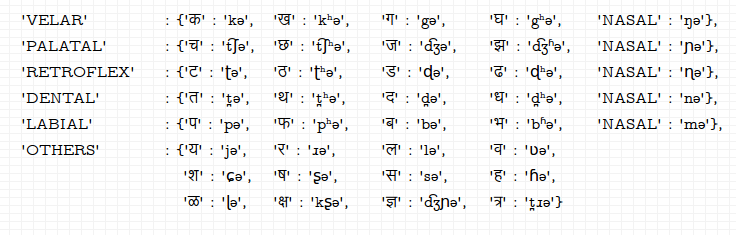
\includegraphics[width=\textwidth]{correspondences.png} 
%		\caption{Sanskrit speech sounds in Devanagari: consonants and non-vowel sounds.}
%	\end{center}
%\end{figure*}


\begin{table}[ht]
	\centering
		
	\begin{center}
		\begin{tabular}{|c|c|c||c|c|c|}
			\hline
			\textbf{Base}&\multirow{1}{*}{\textbf{Diacritic}}&\multirow{1}{*}{\textbf{IPA}}&\textbf{Base} &\multirow{1}{*}{\textbf{Diacritic}}&\multirow{1}{*}{\textbf{IPA}} \\
			%\textbf{glyph}& \textbf{}&\textbf{}&\textbf{glyph}& \textbf{}&{\bf}\\
			\hline%\hline
			\sansk{अ}&&ə& \sansk{आ}& \sansk{ा}&ɑː\\\hline
			\sansk{इ}& \sansk{ि}&i&	\sansk{ई}& \sansk{ी}&iː\\\hline
			\sansk{उ}&\sansk{ ु}&u&
			\sansk{ऊ}& \sansk{ ू}&uː\\\hline
			\sansk{ऋ}&\sansk{ ृ}&ɹ̩&\sansk{ॠ} &\sansk{ ॄ}&ɹ̩ː\\\hline
			\sansk{ऌ}&\sansk{	ॢ}&l̩&\sansk{ॡ} &\sansk{ॣ}&l̩ː\\\hline
			\sansk{ए}&\sansk{ े}&eː& \sansk{ऐ} & \sansk{	ै}&ɑːi\\\hline
			\sansk{ओ}& 	\sansk{ो }&oː&	\sansk{	अाै}&\sansk{ाै}&  ɑːu\\\hline
			\sansk{अं}& \sansk{	ं }&əm&	\sansk{अः}&	\sansk{ः} & əh\\\hline
			\sansk{ॐ} &&oːm&&&%\multicolumn{3}{|c|}{ }
			\\\hline
			
		\end{tabular}
		\caption{Sanskrit speech sounds: vowels and syllabic sounds.}
		\label{vowels-table}
	\end{center}
\end{table}

%\begin{figure*}[!ht]
%	\begin{center}
%		%\fbox{\parbox{6cm}{
%		%This is a figure with a caption.}}
%		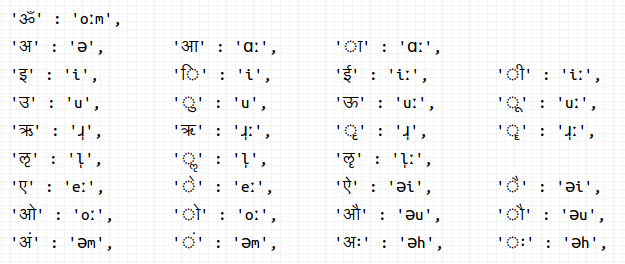
\includegraphics[scale=0.6]{correspondences_vowelsIPA.png} 
%		\caption{Sanskrit speech sounds in Devanagari: vowels and syllabic sounds.}
%	\end{center}
%\end{figure*}


We will base our transcription system upon existing literature on the phonology of Sanskrit \cite{jamison2004sanskrit} as well as a system of correspondences between Devanagari text, IAST, and IPA, in the work `The Original Pronunciation of Sanskrit' \cite{zieba2002original}. We will hence establish a mapping between Devanagari glyphs, their diacritic combinations if any, and IPA symbols \cite{international1999handbook}. Table~\ref{consonants-table} shows the correspondences used for consonants and other non-vowel sounds, while table~\ref{vowels-table} is the vowel and vowel-like sounds' counterpart.
Sanskrit makes use of special symbols for several compound consonants, which we will process using their constituent components. Fortunately, Unicode character combinations for Devanagari define such compound characters in terms of their constituent components by default, making them easier to process.
Although Sanskrit has many complex phonological processes where sounds interact (a popular one of which is \textit{sandhi}), we need not encode rules of such phonetic interaction other than those implied by the orthography. This exclusion is because any phonological combination that occurs (such as from \textit{sandhi}) results into a new phrase, which is written as-is in the orthography. It is expected of an input phrase to be well-formed, i.e., to not have any phonological inconsistencies per the rules of Sanskrit orthography. Given that this program will likely find use in transcription of existing texts, this should not be an issue in most cases.

We have taken the interpretation of sounds to be as close as possible to what is believed to have been the pronunciation in the classical Sanskrit era \cite{zieba2002original,jamison2004sanskrit}. One such noteworthy consideration is the differential pronunciations of a {\it visarga}, or the `\sansk{ः}'-terminal sound. Today, the interpretation of the pronunciation of this sound is slowly shifting towards a new trend: duplicating the vowel sound of the previous syllable after ([{\it \ipa{h}}]). For instance, \sansk{रविः} would end as [-ihi] according this rule as opposed to [-h]. While this seems to be a rising trend, it did not always use to be so,  and the sound was supposed to be simply a {[\ipa{h}]}-terminating one, without vowel duplication.

\section{Rule-Based Transcription}

In our program, we will use several one-pass processes to fully transcribe a given text in linear time. In what follows, we describe some of the orthographic intricacies that require special attention in the design of the program.

\subsection{Shorthand for Nasalization}

The Devanagari Sanskrit orthography has several ways to indicate the presence of a nasal sound. Presence of nasals in a word is semantic, unlike some languages where it may have a conditioned occurrence. Nasals may be one of six types: five, derived from the conventional place of articulation (velar, palatal, retroflex, dental, and labial), and the sixth, simply a nasalized articulation of any vowel. Conventionally, a nasal consonant is only explicitly written when a phrase ends, or if the upcoming character is a vowel.\footnote{As classified in the several tables above. A vowel in the strict phonetic sense is not meant here.} In case the nasal sound is not explicitly shown, an {\it anusvara} is shown on the character preceding it, and the actual sound corresponding to it is inferred from the forthcoming sound at the time of reading. For instance, if a word ends in a nasal sound, and the word after it begins with a bilabial stop, then the nasal is inferred to be [m]. When a sound does not belong to any of the five places of articulation mentioned above (e.g., a fricative, or a vowel), it shall be called the sixth case, and in this case, the preceding vowel is nasalized, with no additional sound being added. For instance, in the word \sansk{संस्कृत} ([sə̃̃s.kɹ̩.t̪ə]), where the {\it anusvara}'s circumstance is not one of the five types mentioned. The specific nasal sound to be used is inferred based on the next sound, if one exists, or is taken to be {[\ipa{m}]}, the bilabial nasal sound, by default.

\subsection{Handling the Default Schwa}

A consonant character in Devanagari Sanskrit, unless explicitly marked {\it halant} (i.e., a schwa-less ``partial'' sound marked using the diacritic \sansk{्}), has an implied schwa. For instance, \sansk{ग} may be transcribed as [ɡə], while to yield [ɡ], we would need to mark a lack of schwa as \sansk{ग्}. Removal of schwa is required when either explicitly marking a character {\it halant}, or when combining it with another vowel, in which case, the vowel combination overrides the schwa. The way Devanagari diacritic combinations work in Unicode are from the point of view of typographic convenience. However, during transcription, we are required to explicitly remove the schwa, as demonstrated in the following example:
\sansk{गो = ग  +  ो}  $\,$ is the way diacritic combination takes place in terms of Unicode characters. However, phonologically speaking, it is $\,$
\sansk{गो = ग + ् + ओ} $\,$([ɡoː]), since we are removing the schwa and explicitly adding another vowel, instead of superficially dealing with diacritical marks. This needs to be taken care of during transcription, since, at the surface level, it is not explicit what underlying phonological process is taking place.


\subsection{Syllabification}

For syllabification, we implement the WWG algorithm \cite{weerasinghe2005rule} adapted to Sanskrit \cite{gdasa2013sanskritSyllabification}. In the original study, the algorithm was developed to account for a majority of the Sinhalese vocabulary which has Sanskrit or Pali origins, as well as a large number of direct borrowings. In the same study, the authors note that the algorithm would be similarly applicable to Sanskrit with some modifications.
As shown in algorithm~\ref{alg1}, we use groups of vowel-consonant-vowel clusters (of the kind $V_BC_nC_{n-1}\dots C_2C_1V_A$, where $n\geq1$) for syllabification. Note that a cluster is not a syllable unit, but simply a device to locate syllable boundaries. We apply rules based on the number of consonants in the middle consonant cluster, i.e., $n$. Based on this length, prosodic syllabification conventions, we mark the boundaries of the syllables.
We reuse boundary vowels, so a vowel that was processed while considering the current cluster will be included again to spot the next cluster. We achieve this by keeping track of indices where clusters began and ended.

\begin{algorithm}[h]
	\label{alg1}
	\SetAlgoLined
	\KwIn{Sanskrit text to be syllabified}
	\texttt{initialize} scope at the beginning of text\;
	\While{end of text not reached}{
		\texttt{move} to next $V_B\mathbb{C}V_A$, where $\mathbb{C}$ is a consonant cluster\;
		\uIf{length of cluster $\mathbb{C} = 1$}{
			\texttt{mark} syllable break after $V_B$\;
		}\uElseIf{length of cluster $\mathbb{C} = 2$}{\texttt{mark} syllable break after first $C$ from left\;}\uElseIf{length of cluster $\mathbb{C} = 3$}{
			\uIf{third consonant from left $=$ \sansk{र् or य्} {\bf or} first and second consonants are stops}{\texttt{mark} syllable break after first $C$ from left\;}
			\uElse{\texttt{mark} syllable break before first $C$ from right\;}
		}\uElse{
			\uIf{first consonant from right $=$ \sansk{र् or य्}}{\texttt{mark} syllable break before second $C$ from right\;}
			\uElse{\texttt{mark} syllable break after least sonorous $C$\;}
			}
	}\KwResult{Syllabified Sanskrit text
	%\vskip0.5em
	}
\caption{WWG Algorithm adapted to Sanskrit}
\end{algorithm}

\subsubsection{Examples}
%\setmainfont{Doulos SIL}
In what follows, we provide some example Sanskrit words to demonstrate syllabification as carried out using algorithm~\ref{alg1}. For ease of reading, we highlight the consonant cluster in consideration using boldface in the Devanagari text.

\begin{enumerate}
	\item \sansk{कृ\textbf{त}म्} ([kɹ̩.t̪əm]) was split before [t̪] following the rule for a cluster of length one.
	
	\item\sansk{व\textbf{ल्क}लानि} ([ˈʋəl.kə.lɑː.ni]): here, the first two syllables have been demarcated from each other by splitting a consonant cluster of length two.
	
	\item 
	\begin{enumerate}
		\item \sansk{म\textbf{त्स्यः}} ([ˈmət̪.sjəh]): this cluster of length three has been split according to the rule that checks the presence of either \sansk{र्} or \sansk{य्}.
		
		\item
		\sansk{उ\textbf{क्त्वा}} ([ˈuk.t̪ʋɑː]) demonstrates the rule involving two stops. Here, \sansk{क् and त्}. Hence, we split it after the first stop from the left hand side.
		
		\item
		\sansk{कृ\textbf{त्स्न}म्} ([ˈkɹ̩t̪s.nəm]) is useful to illustrate the `else' condition when the conditions similar to those in 3(a) and 3(b) do not apply.
	\end{enumerate}
	
	\item
	%\begin{enumerate}
		%\item 
		
		\sansk{का\textbf{र्त्स्न्य}म्} ([kɑːɹt̪s.njəm]) contains a \sansk{य्}-terminal cluster of length more than three. We split it before the second consonant when scanning from the right.
		
		%\item		
	%\end{enumerate}
	
\end{enumerate}
%\setmainfont{FreeSerif}

\subsection{Assigning Stress}
Once we finish demarcating the syllables, we use traditional prosodic and metric rules to determine the syllables that should receive stress. In Sanskrit, a syllable is either `light' ($L$) or `heavy' ($H$) \cite{sridharan2005sanskrit}. A syllable may be considered to be light in the base case, which acquires the status of being heavy subject to meeting one or more of the following conditions.
\begin{enumerate}
	\item Syllable contains a long vowel or diphthong
	\item Syllable is nasal-terminated or has nasalized vowel
	\item Syllable is stressed
\end{enumerate}

The goal is to ensure that any syllable of the form $[C_{11}]V_1[C_{1n}...C_{13}]C_{12}[C_{21}...]V_2$ that results in a cluster of consonants because of the adjoining consonants of the next syllable (here, $C_{21}$ and beyond), is heavy. If the syllable already satisfies at least one of the first two conditions above, it is already heavy. However, if not, we must use condition~3 and add stress to make it into a heavy one.
For the sake of example, consider the syllables of the word \sansk{कुरु{क्षे}त्र} ([ku.ˈɹuk.ʂeː.t̪ɹə]). When taken independently, they have the weights $L,L,H,L$. However, when considered in the word, the character \sansk{क्ष्}, which is a compound consonant of \sansk{क् + ष्}, causes the previous non-heavy syllable (-[.ɹuk.]-) to end into a consonant cluster of consonants of adjoining syllables. It thus receive stress, and hence become heavy, making the weights of syllables $L,H,H,L$. The third syllable does not receive stress, even though the boundary of the syllable break after it, i.e., -[.t̪ɹə], contains a consonant cluster, due to having the long vowel \sansk{े} ([eː]), which satisfies the first condition.

\vspace{.3\baselineskip}

\section{Software}
Prototype software developed as part of this work may be found at the following link:
\hyperref{https://github.com/aalok-sathe/sanskrit_IPA}{}{}{\tt https://github.com/aalok-sathe/sanskrit\_IPA}.

The program is written using Python3, primarily because of effortless inbuilt Unicode support. The program allows the user to transcribe text on-the-go using a command-prompt design. A command in the form: \texttt{transcribe} \textsl{text} may be used. The software can also read an input file externally and output it in a similarly named file. This may be especially useful for transcribing large texts. Specific implementations apart, the software has intuitively named methods and commented code that will allow anyone using it to build software on top.
We observed a lack of permissively licensed software for this purpose, and would like to stress that the prototype program is free and open source software (FOSS) which may be used, modified, and redistributed by anybody in compliance with the GNU General Public License (version 3 or later). It is our hope that this licensing will encourage scrutiny, improvement, and further development in related research questions.

\section{Future Work}
We intend to evaluate the current work against hand-transcribed Sanskrit text. Evaluations will be hosted along with the source code.
More work along similar lines will be required to create a set of tools to represent traditional knowledge in Sanskrit, as well as a large number of Indic languages. To begin with, systems need to be developed that will enable back-transcription from IPA to Devanagari, as well as all-way systems to transcribe consistently to most of the major ways of representing Sanskrit text today, such as ITRANS and IAST.
Whereas developing such a system for Sanskrit is possible using rule-based decision procedures, it is not possible for most other modern Indic languages which rely largely on the speaker's cultural and experiential knowledge of the language for phonetic disambiguation. For such languages as Hindi and Marathi, statistical learning methods will need to be used in addition to rule-based systems to create transcription mechanisms that are accurate.

\section{Acknowledgments}
We are grateful for helpful comments by and discussion with Mukund Gokhale, Hema Kshirsagar, Dieter~Gunkel, Shardul~Chiplunkar, and Thomas Bonfiglio.

%The font Annapurna SIL was used to render Devanagari text for the purpose of this manuscript. This manuscript was typeset using Xe\LaTeX.
% \nocite{*}

\section{Bibliographical References}
\label{main:ref}

\bibliographystyle{lrec}
\bibliography{mybib}


	
%\section{Language Resource References}
%\label{lr:ref}
%\bibliographystylelanguageresource{lrec}
%\bibliographylanguageresource{xample}

\end{document}
